% !TeX spellcheck = en_US
\chapter{Approach}\label{ch:approach}

\section{Definitions}\label{sec:definitions}

This chapter includes some basic definitions that will be used later on.

\subsection{Compression Ratio}

One of the key metrics for a compressor is its compression ratio. The compression ratio depends on the input data and is defined as follows

\begin{align*}
\text{compression ratio} = \dfrac{\text{compressed size}}{\text{original size}} \in (0,1]
\end{align*}

The compression ratio is typically in the $(0,1]$ interval, since the compressed data will not be larger than the original data (there are cases where this happens, but it does not happen in the compressors considered here). Obviously, the compressed data cannot have a size of 0 or less.

Normally the compression ratio is measured at the file size level (in byte). If a different measure is used, it will be mentioned at that point.

\subsection{(De-)Compression Time}

Another key metric of a compressor is its (de-)compression time. This metric also depends on the input data and indicates the run time needed for compression and decompression of the data, respectively. The run time is typically measured in milliseconds.

%\section{Concept}
%
%Fig.~\ref{fig:benchmark_overview} shows the aspects of a benchmark of two compressors. There are parameters that can be set during the evaluation (they start with $p$) and measures that represent the performance of the algorithms (they start with $m$).
%
%The compressors get an input $p_{input}$, which in this case is in RDF graph. They each produce an output $m_{output}$, the compressed data. For compression and decompression there will be run times, which we call $m_{runtime} $. In addition, there are certain parameters $p_{alg}$ that can be set in the algorithms that change the behavior of the algorithm. \todo{hier kommt noch nicht performance von queries vor}
%
%\begin{figure}[h]
%	\centering
%	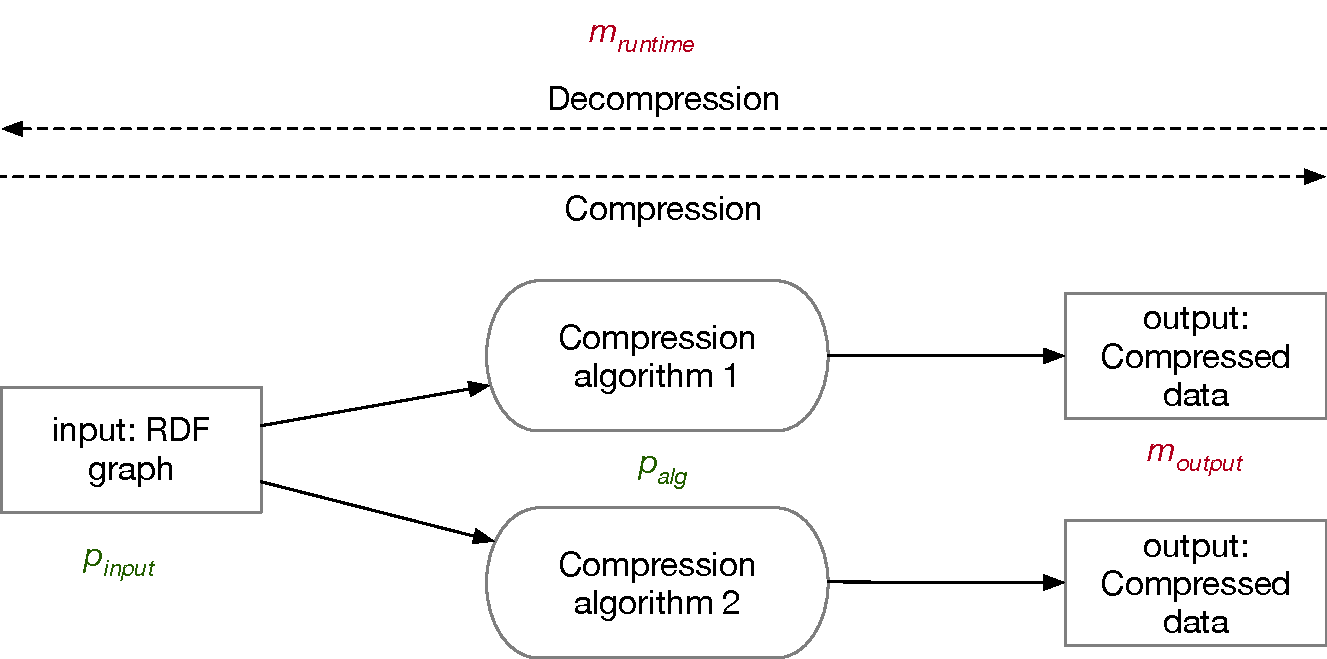
\includegraphics[width=1\textwidth]{figures/approach/Benchmark}
%	\caption{The different aspects of a compression process. $p_{input},p_{alg}$ are parameters that can be changed. $m_{output},m_{runtime}$ are measures of the algorithm's performance.}
%	\label{fig:benchmark_overview}
%\end{figure}

\section{GRP vs HDT}\label{sec:approachGRPvsHDT}

This chapter deals with the comparison between HDT and GRP. The main aim is to determine which of the two compressors achieves a lower compression ratio.

The obvious question is now whether there are certain properties/features that an RDF graph can have, and which have a positive or negative impact on the compression ratio of one or both algorithms. 

\subsection{Relation Between Structure of Data and Compression Ratio}

First these features are considered for HDT. Fig.~\ref{fig:hdt_overview_1} is shown again. There you can see that the size of the data becomes smaller if there are only a few subjects. This is the case because the bit-array $B_p$ contains a 1 every time a new subject is considered. For example, if there is only one subject, then $B_p$ consists only of zeros.

\begin{figure}[h]
	\centering
	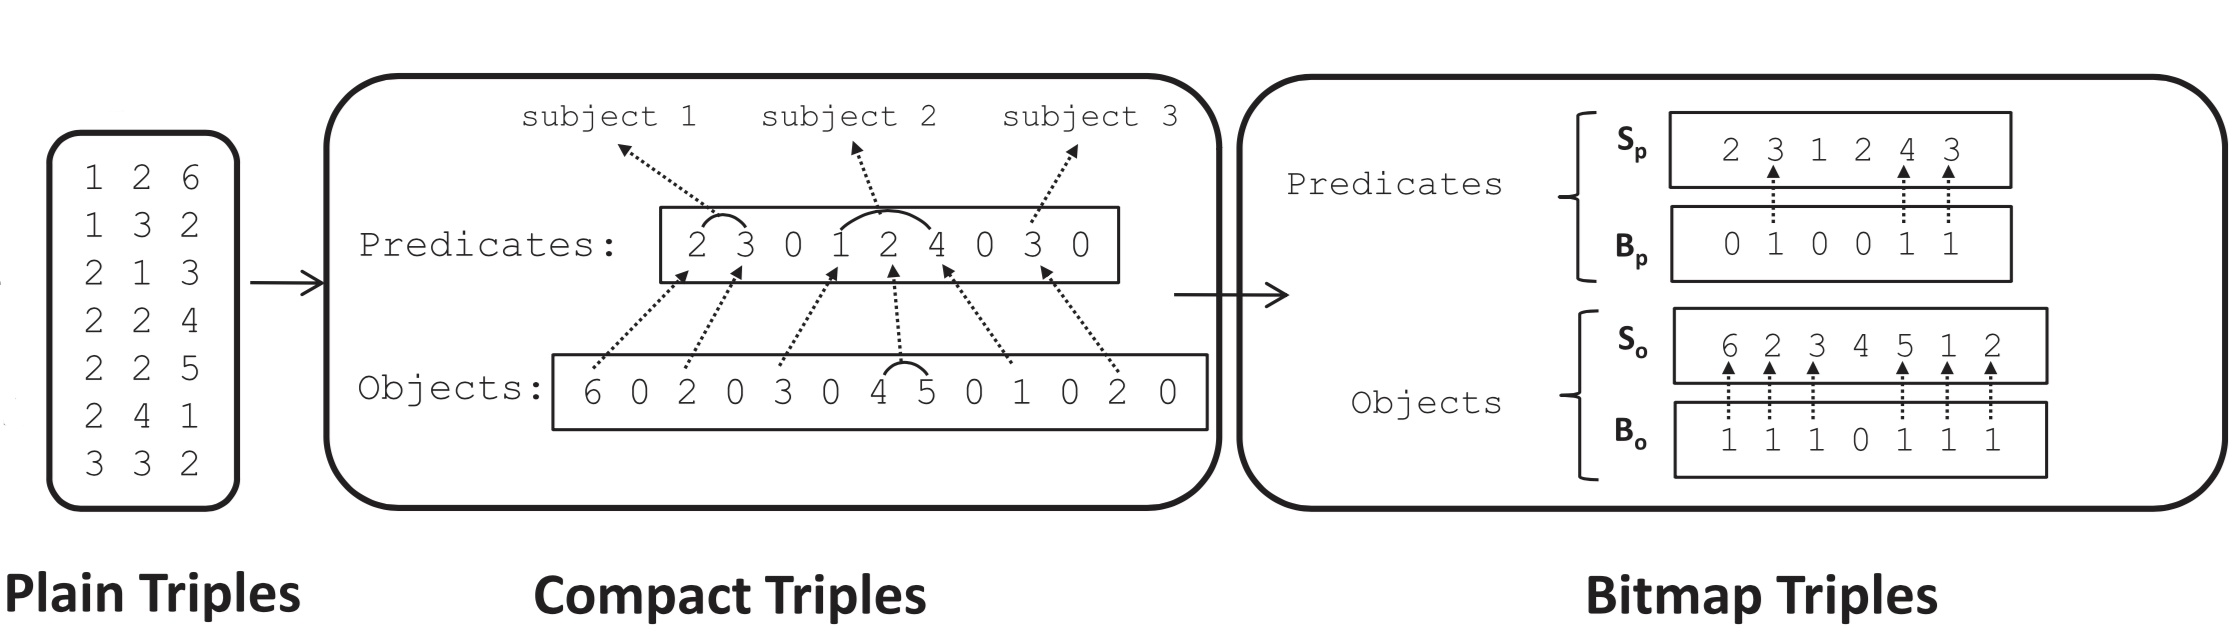
\includegraphics[width=1\textwidth]{figures/relatedwork/hdt1}
	\caption{Three different representations of triples in HDT}
	\label{fig:hdt_overview_1}
\end{figure}

For GRP that feature analysis is more complex. Since GRP constructs grammar rules by using the graph's structure, it is more dependent on the data's structure than HDT. There can be many features that can lead to different constructible grammar rules. Those will not be discussed here. But a simple insight is that GRP's compression ratio will be bigger when there are more different predicates in the graph. This is true, because GRP's grammar rules are based on repeating edge labels. That fact will be considered in the evaluation.

\subsection{Dictionary Size}

As already explained in Ch.~\ref{ch:related_work}, HDT divides an RDF file into its header, dictionary and triples component. This is partially also true for GRP except that GRP does not create a header. But it also assigns an ID to every URI or literal and then only works with these IDs. Unfortunately the authors of~\cite{maneth} did not work on efficient storing of the dictionary. In GRP the size for the dictionary component is just ignored. Therefore we have to add this size in order to compare GRP with HDT in a fair way. To achieve that we just add the same size to the compressed size of GRP that HDT would need to store the dictionary.


\section{Compression Ratio Improvements}\label{sec:approachComprRatioImprovements}

Ch.~\ref{sec:evaluationHDTvsGRP} will show that GRP always achieves a better compression ratio than HDT. Since according to~\cite{maneth} a graph compressed with GRP is less suitable for neighborhood queries (i.e. typical SPARQL queries) than an uncompressed graph, we will concentrate in the following on further improving the compression ratio. So we do not compare the query speeds between HDT and GRP.



\subsection{Ontology Knowledge}\label{sec:approachOntKnowledge}

RDF has meta data that contains knowledge about the actual data. This is also called ontology. An ontology is normally itself an RDF graph. There are two known languages for formulating an ontology: RDFS~\footnote{\label{foot:3}https://www.w3.org/TR/rdf-schema/} and OWL~\footnote{\label{foot:4}https://www.w3.org/TR/2012/REC-owl2-overview-20121211/\#Documentation\_Roadmap}. Of these, OWL is the more powerful and is therefore chosen here.

This chapter is about finding out whether one can change the structure of an RDF graph by applying knowledge from its ontology so that it is more compressible for GRP, but at the same time remains semantically equivalent to the original graph. In this way no data would be lost by compression.

In Ch.~\ref{ch:GRPvsHDT} \todo{fix} it has already been mentioned that GRP depends more on the structure of the input graph than HDT does. It will therefore be interesting to see how applying ontology knowledge influences GRP's compression ratio.

This chapter is about elaborating the theoretical concepts of OWL and investigating how they can be used for grammar-based compression.

Let \[ elr = \dfrac{\text{number of different edge labels}}{\text{number of edges}} \] (edge label ratio) be the ratio of the edge labels or properties to the total number of edges of the graph. 

Generally it can be said that GRP can compress a graph better if $elr$ is lower, because then there is more redundancy in the graph. However, if the graph structure becomes unfavorable for GRP, the compression ratio may still be worse at a lower value for $elr$.


\subsubsection{Symmetric Properties}

There is a predicate in OWL called \enquote{owl:SymmetricProperty} which expresses that a certain other predicate $p$ is symmetric. This means, if there is a triple $(s,p,o)$ in the graph, then there can also be a triple $(o,p,s)$ at the same time. In reality, however, it can happen that only one of the two triples really exists in the graph. The idea now is to always add the other triple to the graph in such a case. This makes the graph larger at first, but more grammar rules can be found. Das liegt daran, dass man durch das Hinzufügen $elr$ kleiner macht, was grundsätzlich schon mal zu einer besseren Kompressionsrate führen kann. Gleichzeitig sollte es dabei aber nicht zu einer ungünstigen Struktur kommen:

\todo{bild und erklärung}


\subsubsection{Transitive Properties}

\subsubsection{Inverse Properties}

\subsubsection{Equivalent Properties}


\subsection{Dictionary Improvements}\label{sec:approachDictImprovements}


As already seen in Ch.~\ref{ch:GRPvsHDT}, the dictionary makes up most of the memory of a compressed RDF graph. It is therefore worth investigating whether the dictionary can be compressed better. One can take advantage of certain features of the dictionary to achieve that.

As mentioned above, GRP does not have its own method for compressing the dictionary. We have therefore taken the compression method from HDT, and applied it in GRP to ensure a fair comparison.

HDT has a fairly mature mechanism for compressing the dictionary.\todo{genauer erklären}

\subsubsection{Literals}\label{sec:approachLiterals}

Objects in RDF can be literals. Literals typically contain constant values and usually have no common prefixes. Therefore the compression of HDT is not suitable for these. Since literals can often contain whole flow texts, a text compression would probably be well applicable. An example of such a text compression is a Huffman Code~\cite{huffman}. Here the text is converted into a binary format. Every single character of a text is binary coded, whereby frequently occurring characters get short and rare characters get longer codes. These codes are expressed by a binary Huffman tree. An example can be seen in Fig.~\ref{fig:huffmantree}. Each leaf contains a symbol whereas the one and zeros on the path to the symbol define its code. The tree is constructed in such a way that paths to frequent characters are shorter than those to rare characters. The whole procedures can be seen in~\cite{huffman}.

This tree must then be stored in addition to the compressed data so that the original data can be recovered. It will be seen in Ch.~\ref{ch:implementation} how that is done.

\subsubsection{Blank Nodes}\label{sec:approachBlankNodes}

Blank nodes are normally used when a node does not get a URI, but is still necessary to represent a statement. Such a node is often used to formulate more complex logical statements. The same blank node can occur in different triples. In order for it to be referenced uniquely, it gets an ID. These IDs are usually chosen arbitrarily and have no meaning beyond that. When reading an RDF graph with the Jena-API~\footnote{\label{foot:5}https://jena.apache.org/index.html} (which is used by HDT) random UUID strings are assigned for the blank nodes, which are quite long. They also have no common prefixes, which makes the HDT dictionary compression ineffective again. 

To improve compression, one can reassign the IDs of the blank nodes. For example you can use numbers from 1 to $n$ ($n=$ number of blank nodes) to have short IDs. 

Another possibility is not to save the IDs of the blank nodes at all. In HDT all strings in the dictionary (including the blank node IDs) are mapped to short IDs. Thus the blank node IDs are in principle already stored. They can therefore be removed from the dictionary. HDT must then be changed so that it can handle the case in which it does not find a corresponding string in the dictionary for a certain short ID. At this point it would know directly that the considered node is a blank node and the longer blank node ID is unimportant. Such a situation will occur when a decompression is performed.

In Ch.~\ref{sec:evalDict} one can see the effects of shortening and becoming blank node IDs on the compression ratio.















